\documentclass{homework}

\title{Homework 4}
\author{Kevin Evans}
\studentid{11571810}
\date{February 10, 2021}
\setclass{Physics}{465}
\usepackage{amssymb}
\usepackage{mathtools}
\usepackage{graphicx}
\usepackage{amsthm}
\usepackage{amsmath}
\usepackage{slashed}
\usepackage{boldline}
\usepackage{physics}
\usepackage{tcolorbox}
\usepackage[inter-unit-product =\cdot]{siunitx}

\usepackage[makeroom]{cancel}
\usepackage{booktabs}
\usepackage{multirow}

\usepackage{times}
\usepackage{mhchem}
\usepackage{enumitem}
\usepackage[normalem]{ulem}
\usepackage{systeme}
\usepackage{tikz}
\usepackage{mathtools}
\usepackage{tabularx}

%\usepackage{calligra}
%\DeclareMathAlphabet{\mathcalligra}{T1}{calligra}{m}{n}
%\DeclareFontShape{T1}{calligra}{m}{n}{<->s*[2.2]callig15}{}
%\newcommand{\scriptr}{\mathcalligra{r}\,}
%\newcommand{\boldscriptr}{\pmb{\mathcalligra{r}}\,}
%\newcommand{\emf}{\mathcal{E}}

\DeclareSIUnit\eVperc{\eV\per\clight}
\DeclareSIUnit\clight{\text{\ensuremath{c}}}
\DeclareSIUnit\year{yr}

\newcommand{\fm}{\femto\meter}

\begin{document}
	\maketitle
	\begin{enumerate}
		\item Using the uncertainty principle, \begin{align*}
			\Delta x \Delta p & = \hbar / 2 
			\intertext{For a well of radius $\SI{2}{\fm}$,}
			\Delta p & = \hbar / 2 / (\SI{2}{\fm}) \\
				& \approx \SI{50}{\MeV/c}.
		\end{align*}
		As the electron rest mass is minuscule, the electron would require a massive binding energy.
	
		\item For a nucleon, it's rest mass is roughly \SI{1}{\GeV/c^2}, must larger than the kinetic energy from $p=\SI{50}{\MeV/c}$. As it would be non-relativistic, we can assume \begin{align*}
			E & = p^2 / 2m = (\SI{50}{\MeV/c})^2 / (2 \times \SI{1}{\GeV/c^2}) \\
				& \approx \SI{1.25}{\MeV}.
		\end{align*}
		This binding energy is much less than that required of an electron.
		
		\item \begin{enumerate}
			\item Is it because when a neutron is in a nucleus, it's trapped in a well and it is energetically unfavorable to decay (I assume it has to overcome the Coulombic (p-p) and the increase in energy due to taking a higher energy state due to the Pauli exclusion principle)? Whereas, when the neutron is alone, there isn't anything keeping it from decaying. 
			
			\item Because the kinetic energy of the proton and electron pair must be balanced with the rest mass change $Q$, \begin{align*}
				T & = \frac{p^2}{2m_p} + \frac{p^2}{2m_e} = Q \\
					& = m_n c^2 - m_pc^2 - m_e c^2.
			\end{align*}
			If there's a smooth spectra of energies in the $\beta$-particles, there must be another particle that can also take a smooth spectra of energies, like the neutrino. 
		\end{enumerate}
	
		\item \begin{enumerate}
			\item As $Z$ increases, there is greater p-p repulsion and requires more neutrons to ``space'' them out and reduce Coulomb effects.
			
			\item It's because more neutrons are needed for Coulombic stability in heavy elements. During fission of heavy elements, there is then an excess of neutrons as the atoms are split to its daughter products. This results in $\alpha$ decay, and $\beta$-decay where a neutron is ``converted'' to a proton.
		\end{enumerate}
	
	\pagebreak
	
		\item \begin{enumerate}
			\item \begin{itemize}
				\item $a_v A$: the volume binding term---this uses $A$ as it's roughly proportional to the volume
				\item $-a_s A^{2/3}$: the surface ``tension'' energy term, this relies on the surface area, proportional to $r^2 \implies A^{2/3}$
				\item $-a_c \dfrac{A^2}{A^{1/3}}$: the Coulombic term from proton-proton interaction, proportional to $Z$ and relies on $r \implies A^{1/3}$
			\end{itemize}
		
			\item The asymmetry term arises from the Pauli exclusion principle and is governed by strong force interaction. If we exchange a pair of protons for a pair of neutrons, the energy of the neutrons must be higher, as it can only sit in the next ``rung'' of the potential well (due to the exclusion principle). Each additional layer requires an additional energy proportional to the current energy, i.e. the current imbalance of protons to neutrons, similar to a spring force. From in-class, this means \begin{align*}
				\dd{E} & = (Z-N) \dd{(Z-N)} \\
				\implies E & \propto (Z-N)^2 / 2.
			\end{align*}
			
			
			This image is from Wikipedia, but I think it well describes the increased energy due to the Pauli principle. For an atom with $A=16$ nucleons, if there is no difference in the count of protons and neutrons, the energy is then lower. If there are more neutrons than protons, the energy is higher.
			
			\begin{center}
				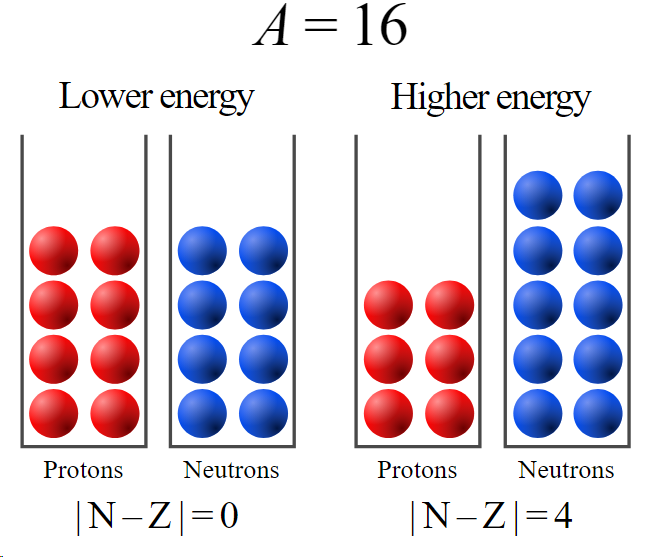
\includegraphics[width=0.7\linewidth]{screenshot001}
			\end{center}
			
			
		\end{enumerate}
	\end{enumerate}
\end{document}